\section{Durchführung}
\label{sec:Durchführung}

Der Aufbau des Experiments ist in Abb. \ref{fig:aufbau} zu erkennen. In einem Glaszylinder befinden sich ein $\symup{\alpha}$-Präparat (Americium), welches als Strahlungsquelle dient, und ein Detektor. Der Abstand zwischen Präparat und Detektor lässt sich mittels eines verschiebbaren Halters ändern. Der Detektor ist ein Halbleiter-Sperrschichtzähler, der ähnlich einer Diode aufgebaut ist. 
Zur Messung wird das Programm Multichannal Analyzer benutzt. 

\begin{figure}
    \centering
    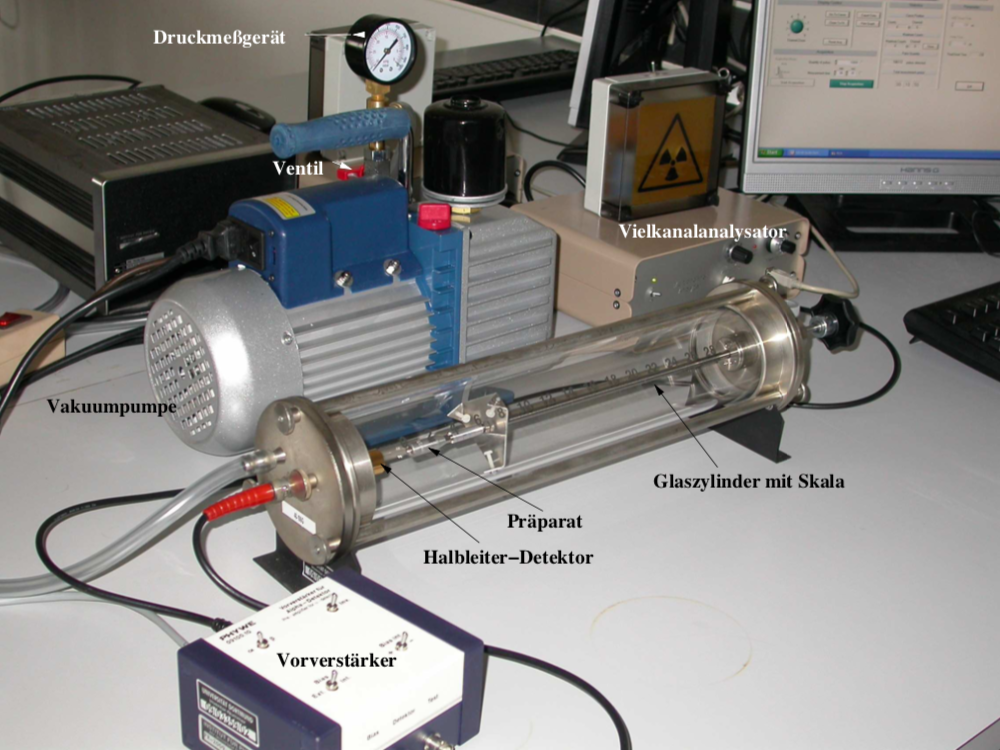
\includegraphics[width=10cm, height=8cm]{build/aufbau.png}
    \caption{Zu sehen ist der Versuchsaufbau zur Messung der Reichweite von $\symup{\alpha}$-Strahlung. \cite{V701}}
    \label{fig:aufbau}
\end{figure}

\subsection{Messung des Energieverlustes von Alphastrahlung in Luft}
Es wird der Energieverlust von $\symup{\alpha}$-Strahlung in Luft untersucht.
Es sollen die Energieverteilung und die Zählrate der $\symup{\alpha}$-Strahlung in Abhängigkeit des Drucks bestimmt werden.
\newline
Dazu wird der Abstand zwischen Präparat und Detektor zunächst auf $d_1 = \SI{2.7}{\centi\meter}$ gestellt. Der Glaszylinder wird evakuiert ($\SI{0}{\bar}$). Anschließend wird der Druck in $\SI{50}{\milli\bar}$ Schritten auf $\SI{1000}{\milli\bar}$ erhöht und jeweils die Anzahl der detektierten Pulse und die Position des Energiemaximums nach $\SI{120}{\second}$ Messzeit aufgenommen.
\newline
Die ganze Messung wird für einen Abstand $d_2 = \SI{2}{\centi\meter}$ wiederholt.

\subsection{Untersuchung der Statistik des radioaktiven Zerfalls}
Im letzten Schritt wird die Statistik des radioaktiven Zerfalls überprüft, indem bei evakuiertem Glaszylinder die Zerfälle in $\SI{10}{\second}$ $\num{100}$ mal gemessen werden. Der Detektor ist dabei $\SI{3}{\centi\meter}$ vom Präparat entfernt.